% Final report (8 pages) - FAI Group 22. Extends the project-review submission (proposal/project_proposal.tex)
% with Methodology, Results and Contribution sections, in the same template.
% Compile from this directory: pdflatex final_report && pdflatex final_report   (arxiv.sty is here)
% Every number is recomputed from results/sweep_*/summary.csv by `python report_numbers.py`
% (run from the repository root); figures come from `python run_evaluation.py report ...`.
\documentclass{article}

\usepackage{arxiv}
\usepackage[utf8]{inputenc}
\usepackage[T1]{fontenc}
\usepackage{hyperref}
\usepackage{url}
\usepackage{booktabs}
\usepackage{amsfonts,amsmath,amssymb,amsthm}
\usepackage{microtype}
\usepackage{graphicx}
\usepackage[numbers,sort&compress]{natbib}
\usepackage{algorithm}
\usepackage{algpseudocode}
\usepackage{enumitem}
\usepackage{tabularx}
\usepackage{dsfont}
\usepackage{caption}

\captionsetup{font=small,labelfont=bf,skip=4pt}
\setlist{nosep,leftmargin=*}
\setlength{\textfloatsep}{10pt plus 2pt minus 2pt}
\setlength{\floatsep}{8pt plus 2pt minus 2pt}

\theoremstyle{definition}
\newtheorem{assumption}{Assumption}
\newcommand{\R}{\mathbb{R}}
\newcommand{\N}{\mathbb{N}}
\newcommand{\E}{\mathbb{E}}
\newcommand{\ind}[1]{\mathds{1}\!\left[#1\right]}
\newcommand{\Reg}{\mathrm{Reg}}
\newcommand{\Eff}{\mathrm{Eff}}
\newcommand{\BR}{\mathrm{BR}}

\title{Learning to Bid Under a Budget: A Batched First-Price Ad Auction with Unknown Click Probabilities}

\renewcommand{\headeright}{Final Report}
\renewcommand{\undertitle}{Final Report --- CS329 Foundations of AI, Group 22}
\renewcommand{\shorttitle}{Learning to Bid Under a Budget}

\author{
  Vivek Raj \\ IIT Gandhinagar \\ \texttt{23110362@iitgn.ac.in} \And
  Anvit Aggarwal \\ IIT Gandhinagar \\ \texttt{anvit.aggarwal@iitgn.ac.in} \And
  Eshaan Ashish Jaiswal \\ IIT Gandhinagar \\ \texttt{eshaan.jaiswal@iitgn.ac.in} \And
  Gella Naga Sai Krishna \\ IIT Gandhinagar \\ \texttt{gella.saikrishna@iitgn.ac.in}
}
\date{}

\hypersetup{
  pdftitle={Learning to Bid Under a Budget: Final Report},
  pdfauthor={Vivek Raj, Anvit Aggarwal, Eshaan Ashish Jaiswal, Gella Naga Sai Krishna},
}

\begin{document}
\maketitle

\begin{abstract}
Budget-constrained advertisers repeatedly buy impressions in a batched first-price auction. Each round
they submit one integer bid per user, subject to a budget, without knowing how likely each user is to
click. With known click probabilities the best response is a $0$--$1$ knapsack, which we solve exactly
and use to compute reference equilibria (Tier~1). We then let one advertiser learn against fixed
equilibrium opponents (Tier~2) and let all advertisers learn at once (Tier~3). A shared evaluation
harness measures regret, equilibrium gap, allocation efficiency, profit and revenue over $30$ seeds with
$95\%$ confidence intervals, across $48$ market sizes ($m\in\{2,3,5\}$ advertisers, $n\in\{5,\dots,50\}$
users, four budget levels) and three budget structures. Thompson sampling has the lowest regret in all
$47$ Tier-2 cells that admit a pure equilibrium, with regret growing as $T^{0.33}$ at $T=10^3$ and
$T^{0.2}$ at $T=10^4$. When all advertisers learn, the market stays away from equilibrium by an amount
that grows with $m$; with Thompson sampling, nearly all of that gap is already present when click
probabilities are known.
Scarce budgets reduce efficiency through the equilibrium itself, not by slowing learning.
\end{abstract}

\keywords{Multi-agent systems \and Auction theory \and Multi-armed bandits \and Knapsack-constrained bidding \and Online advertising}

% =====================================================================
\section{Introduction}\label{sec:intro}
Online ad platforms sell many impressions at once to advertisers with fixed budgets, who can learn a
user's click rate only by winning that user. Budgets turn this into an allocation
(knapsack) problem~\citep{kellerer2004knapsack}; unknown click rates add the exploration--exploitation
dilemma of multi-armed bandits~\citep{auer2002finite,lattimore2020bandit}; and the first-price rule,
which many exchanges now use, makes the price of a user depend on what competitors bid~\citep{krishna2009auction}.
Single-bidder learning in repeated auctions with budgets is well studied~\citep{balseiro2019learning,han2020optimal},
as are bandits with knapsacks~\citep{badanidiyuru2013bandits} and combinatorial semi-bandits~\citep{chen2013combinatorial},
but the interaction of several \emph{simultaneously learning}, budget-limited bidders is less understood.

\paragraph{Guiding question.} \emph{How much worse off are advertisers, and how much less efficient is the
allocation, when click probabilities must be learned online rather than known, and how does this gap
change when all advertisers learn at the same time?}

\paragraph{What we did.} We relax one assumption at a time. \textbf{Tier~1} assumes known click
probabilities and computes exact best responses and reference equilibria. \textbf{Tier~2} gives one
advertiser a bandit learner against opponents fixed at the Tier-1 equilibrium, a stationary single-agent
problem. \textbf{Tier~3} lets all advertisers learn concurrently, so each faces a non-stationary market.
Our contributions are (i)~an exact knapsack formulation of the per-round best response and its use as the
optimisation oracle inside every learner (Section~\ref{sec:method}); (ii)~five budget-aware learners and a
known-$f$ control, all run through one shared simulator and metric pipeline; and (iii)~a $30$-seed study
over $48$ market sizes, three budget structures and two horizons, with every reported number reproducible
from the repository (Section~\ref{sec:results}). Following the TA's review of our proposal, we kept the
scope to the three tiers and shortened future work to a paragraph.

% =====================================================================
\section{Problem formulation}\label{sec:model}
Advertisers $A=\{a_1,\dots,a_m\}$ compete for a fixed, known set of users $U=\{u_1,\dots,u_n\}$ over
$T$ rounds. User $u_j$ clicks $a_i$'s ad with unknown probability $f_{ij}\in[0,1]$; a click is worth $v>0$.
Advertiser $a_i$ has an integer budget $B_i$.

\paragraph{Strategies, allocation, payments.} In round $t$, $a_i$ submits a bid vector from
$S_i=\{b_i\in\{0,\dots,B_i\}^n:\sum_j b_{ij}\le B_i\}$ (Assumption 1 of the proposal: integer bids, so
every $S_i$ is finite). On each user the highest positive bid wins, ties are broken uniformly at random,
and the winner pays its own bid whether or not the user clicks. Let $c_{-i,j}=\max_{k\ne i}b_{kj}$ be the
highest competing bid and $M_{-i,j}$ the number of opponents tied with $b_{ij}$. The probability that
$a_i$ wins $u_j$ is $q_{ij}(b)=1$ if $b_{ij}>c_{-i,j}$, $1/(1+M_{-i,j})$ if $b_{ij}=c_{-i,j}>0$, and $0$
otherwise. A won impression yields a click $X_{ij}\sim\mathrm{Ber}(f_{ij})$, and the expected profit,
platform revenue and expected welfare are
\begin{equation}\label{eq:profit}
  p_i(b)=\sum_{j} q_{ij}(b)\big(f_{ij}v-b_{ij}\big),\qquad
  \mathrm{Rev}(b)=\sum_{i,j}q_{ij}(b)\,b_{ij},\qquad
  \mathrm{Wel}(b)=\sum_{i,j}q_{ij}(b)\,f_{ij}v .
\end{equation}

\paragraph{Feedback.} After each round $a_i$ observes the click $X^t_{ij}$ only on users it won
(semi-bandit feedback), and the highest competing bid $c^t_{-i,j}$ on every user (Assumption~2 of the
proposal). A learning policy maps $a_i$'s own history to a bid vector in $S_i$.

\paragraph{Round structures.} \emph{Canonical} (the main model): the budget resets every round and the
objective is $\E\sum_{t\le T}p_i(b^t)$. \emph{Discounted}: as canonical, with round $t$ weighted by
$\gamma^{t-1}$. \emph{Cumulative}: one campaign budget shared by all rounds, which turns the problem into
bandits with knapsacks~\citep{badanidiyuru2013bandits}.

\paragraph{Best response is a knapsack.} Fix $c_{-i}$. Bidding $c_{-i,j}+1$ wins $u_j$ outright, and any
lower positive bid wins nothing except at a tie, so (ignoring ties) the best response picks a set of users
$x\in\{0,1\}^n$:
\begin{equation}\label{eq:knap}
  p_i^\ast(c_{-i})=\max_{x\in\{0,1\}^n}\ \sum_j \underbrace{\big(f_{ij}v-c_{-i,j}-1\big)}_{r_{ij}}x_j
  \quad\text{s.t.}\quad \sum_j \underbrace{(c_{-i,j}+1)}_{w_{ij}}x_j\le B_i ,
\end{equation}
with bids $b_{ij}=(c_{-i,j}+1)x_j$. This is a $0$--$1$ knapsack with integer weights. Because bids are
integers, the cheapest win costs $1$, so with the normalisation $v=1$ every item value $f_{ij}-c_{-i,j}-1$
is non-positive and no one ever bids. We therefore set $v=5$ in all experiments: a win at price $1$ is
profitable whenever $f_{ij}>0.2$.

% =====================================================================
\section{Methodology}\label{sec:method}
All tiers share one auction engine (\texttt{src/env/auction.py}), one agent interface
(\texttt{get\_bid}, \texttt{observe}, \texttt{reset}) and the knapsack solver below. Agents never see the
true $f$; only the evaluator uses it.

\subsection{Exact best response by dynamic programming}\label{sec:dp}
Items with $r_{ij}\le0$ or $w_{ij}>B_i$ are dropped. Over the remaining items, $D[k][\beta]$ is the best
value using the first $k$ items with capacity $\beta$:
$D[k][\beta]=\max\{D[k-1][\beta],\ D[k-1][\beta-w_k]+r_k\}$ (second term only when $w_k\le\beta$), with
$D[0][\cdot]=0$. A boolean table records which branch was taken, and backtracking from $D[n][B_i]$ recovers
$x^\ast$. This takes $O(nB_i)$ time and memory (\texttt{src/tier1/knapsack.py}). The best response used in
equilibrium computation also compares the knapsack bids with the all-zero bid under the exact
tie-aware utility~\eqref{eq:profit} and keeps the better one.

\subsection{Tier 1: reference equilibria and the planner}\label{sec:tier1}
The game $(A,\{S_i\},\{p_i\})$ is finite, so a mixed equilibrium exists~\citep{nash1951noncooperative}.
We need one reference profile $b^\ast$ per instance, certified by the equilibrium gap
$\varepsilon(b)=\max_i\big(\BR_i(b_{-i})-p_i(b)\big)$, which costs $m$ knapsack solves.
Algorithm~\ref{alg:tier1} shows the solver (\texttt{src/tier1/equilibrium.py}): exhaustive search over pure
profiles for small games, otherwise round-robin best-response dynamics (BRD) from the all-zero profile,
keeping the lowest-gap profile seen. The fictitious-play fallback best-responds to a $20$-sample estimate of
the opponents' empirical mixture for $150$ rounds. An instance is labelled \emph{pure} when the returned
profile has $\varepsilon\le10^{-6}$ ($10^{-4}$ if it comes from fictitious play). This is a \emph{restricted}
notion: no advertiser gains by a deviation that bids $c_{-i,j}+1$ or $0$ on each user. An exact best response
over all of $S_i$, which may also tie a rival's bid (\texttt{check\_tie\_deviations.py}), improves on $62\%$ of
these profiles (median gain $8\%$ of an advertiser's profit; $18\%$ of profiles at $\kappa=0.1$, $99\%$ at
$\kappa=1$). Our learners also bid only $c_{-i,j}+1$ or $0$, so regret and gap compare like with like.
The \emph{social planner} assigns each user to $\arg\max_i f_{ij}$, which upper-bounds welfare
(\texttt{src/tier1/social\_planner.py}).

\begin{algorithm}[t]
\caption{Tier-1 reference profile $b^\ast$ (known $f$)}\label{alg:tier1}
\small
\begin{algorithmic}[1]
\Function{BR}{$i$, $b_{-i}$}\Comment{exact best response}
  \State $c_{-i,j}\gets\max_{k\ne i}b_{kj}$;\ \ $r_j\gets f_{ij}v-c_{-i,j}-1$;\ \ $w_j\gets c_{-i,j}+1$
  \State $x^\ast\gets$ \textsc{KnapsackDP}$(w,r,B_i)$;\ \ $b_i\gets(w_jx^\ast_j)_j$
  \State \Return $\arg\max\{p_i(b_i,b_{-i}),\ p_i(\mathbf 0,b_{-i})\}$
\EndFunction
\Function{Gap}{$b$}\ \Return $\max_i\big(p_i(\textsc{BR}(i,b_{-i}),b_{-i})-p_i(b)\big)$\EndFunction
\If{$m\le3$, $n\le5$ and $\prod_i|S_i|\le5\cdot10^4$}
  \State $\mathcal E\gets\{b\in S:\textsc{Gap}(b)\le10^{-6}\}$ \Comment{exhaustive pure-profile search}
  \State \Return $\arg\max_{b\in\mathcal E}\mathrm{Wel}(b)$ if $\mathcal E\neq\emptyset$, else $\arg\min_{b\in S}\textsc{Gap}(b)$
\EndIf
\State $b\gets\mathbf 0$;\ \ $b^\ast\gets b$
\For{$k=1,\dots,100$}\Comment{best-response dynamics}
  \For{$i=1,\dots,m$} $b_i\gets\textsc{BR}(i,b_{-i})$\EndFor
  \If{$\textsc{Gap}(b)<\textsc{Gap}(b^\ast)$} $b^\ast\gets b$\EndIf
  \If{$\textsc{Gap}(b)\le10^{-6}$} \textbf{break}\EndIf
\EndFor
\State If $\textsc{Gap}(b^\ast)>10^{-6}$ and $m\le3$, $n\le6$: run fictitious play, keep the lower-gap profile
\State \Return $b^\ast$
\end{algorithmic}
\end{algorithm}

\subsection{Tiers 2 and 3: budget-aware learners}\label{sec:learners}
Every learner is a combinatorial semi-bandit: each user is an arm, the knapsack~\eqref{eq:knap} is the
combinatorial constraint, and only won users give feedback. Algorithm~\ref{alg:learner} is the common
template (\texttt{src/tier2/agents.py}). The learner keeps, per user, the number of won impressions $N_j$
and clicks $s_j$. Round~1 is a zero-bid probe that reveals $c_{-i}$ at no cost. From round~2 it replaces
$f_{ij}$ in~\eqref{eq:knap} with an index $\tilde f_j$ and $c_{-i}$ with the last observed competing bids,
solves the knapsack, and bids $\hat c_{-i,j}+1$ on the chosen users. The learners differ only in
$\tilde f_j$:
\begin{itemize}
  \item \textbf{UCB}: $\tilde f_j=\min\{1,\ s_j/N_j+\sqrt{\alpha\ln t/N_j}\}$, and $1$ if $N_j=0$. Default
        $\alpha=2$ (UCB1~\citep{auer2002finite}); we also test $\alpha\in\{0.5,1\}$.
  \item \textbf{Thompson sampling (TS)}: $\tilde f_j\sim\mathrm{Beta}(1+s_j,\ 1+N_j-s_j)$, one fresh
        sample per user per round~\citep{thompson1933likelihood,agrawal2012analysis}.
  \item \textbf{Greedy}: $\tilde f_j=s_j/N_j$, and $1$ for unvisited users (no exploration bonus).
        \textbf{$\epsilon$-greedy}: greedy, except that with probability $\epsilon=0.1$ the round buys a
        random feasible set (users shuffled, added while the budget allows).
  \item \textbf{Budget-paced} (for the cumulative structure): a UCB learner with a dual price
        $\lambda_t\ge0$ on spending. Item values become $\tilde f_jv-(1+\lambda_t)w_j$, the capacity is
        $\min\{\text{remaining budget},\,B_i,\,\max(1,2\lceil\text{remaining}/\text{rounds left}\rceil)\}$,
        and after each round $\lambda_{t+1}=\max\{0,\lambda_t+\eta(\text{spend}_t-\text{total}/T)\}$ with
        $\eta=1/\sqrt T$. This is a Lagrangian approximation of the fluid LP of bandits with
        knapsacks~\citep{badanidiyuru2013bandits,agrawal2014bandits}. Under per-round budgets it
        receives total budget $B_iT$, so its spend never exceeds the target pace, $\lambda_t$ stays $0$,
        and it coincides with UCB.
\end{itemize}

\begin{algorithm}[t]
\caption{Budget-aware semi-bandit bidding for advertiser $a_i$ (Tiers 2 and 3)}\label{alg:learner}
\small
\begin{algorithmic}[1]
\State $N_j\gets0$, $s_j\gets0$ for all $j$;\ \ $\lambda\gets0$
\For{$t=1,\dots,T$}
  \If{$t=1$} bid $\mathbf 0$ \Comment{free probe: reveals $c^1_{-i}$}
  \Else
    \State $\hat c_{-i,j}\gets c^{t-1}_{-i,j}$;\ \ $w_j\gets\hat c_{-i,j}+1$
    \State $\tilde f_j\gets$ UCB index, Beta sample, or $s_j/N_j$ (learner-specific)
    \State $r_j\gets\tilde f_jv-(1+\lambda)w_j$ \Comment{$\lambda\equiv0$ except for the paced learner}
    \State $x\gets$ \textsc{KnapsackDP}$(w,r,\text{capacity})$ \Comment{$\epsilon$-greedy: random feasible set w.p.\ $\epsilon$}
    \State bid $b_{ij}=w_jx_j$
  \EndIf
  \State Observe $c^t_{-i,j}$ for all $j$; for each won $j$: $N_j\gets N_j+1$, $s_j\gets s_j+X^t_{ij}$
  \State Paced only: update remaining budget and $\lambda\gets\max\{0,\lambda+\eta(\text{spend}_t-\text{total}/T)\}$
\EndFor
\end{algorithmic}
\end{algorithm}

\paragraph{Tier 2.} Advertiser $a_1$ runs a learner and $a_2,\dots,a_m$ play $b^\ast_{-1}$. The competing
bids are then constant, so after the probe $\hat c_{-1}$ is exact and only $f_{1\cdot}$ must be learned.
Instances whose Tier-1 profile is not a certified pure equilibrium are excluded from Tier~2.

\paragraph{Tier 3.} All $m$ advertisers run the same learner (\texttt{src/tier3/simulation.py}). Each now
plans against last round's bids while the others change theirs, so the environment is non-stationary and
no single-agent regret guarantee applies. As a control, \texttt{oracle\_br} gives every advertiser the
true $f$ and has it best-respond to last round's bids. This is simultaneous best-response dynamics with
learning removed, and it separates the effect of concurrent adaptation from the effect of not knowing $f$.

\subsection{Evaluation harness and metrics}\label{sec:harness}
The harness (\texttt{src/eval/}) instantiates agents by registry name, runs the round loop with the shared
auction engine, and computes per-round metrics in vectorised form with the true $f$. An infeasible bid
vector is replaced by zeros and counted; this only happens under cumulative budgets, when an agent that
does not track its campaign budget bids more than it has left. For profile $b^t$:
\begin{itemize}
  \item \textbf{Regret} $\Reg^{(i)}_T=\sum_t\big(p_i^\ast(c^t_{-i})-p_i(b^t)\big)$ against the
        knapsack value~\eqref{eq:knap} at the competing bids actually played. We summarise its growth by
        the least-squares slope of $\log\Reg_t$ on $\log t$ for $t\ge T/10$ (the \emph{regret exponent}:
        $1$ is linear, $0.5$ is $\sqrt T$-type, smaller is slower; a fitted slope, not a proven rate). Under cumulative budgets the
        benchmark is the fluid LP: per round, the fractional-knapsack value at capacity total$/T$.
  \item \textbf{Equilibrium gap} $\varepsilon_t=\max_i\max\{0,\ p_i^\ast(c^t_{-i})-p_i(b^t)\}$ and
        distance $\|b^t-b^\ast\|_1$.
  \item \textbf{Allocation efficiency} $\Eff_t=\frac1n\sum_j\sum_{i\in\arg\max_k f_{kj}}q_{ij}(b^t)$:
        the expected share of users won by their highest-value advertiser.
  \item \textbf{Revenue}, \textbf{welfare}, \textbf{total profit}, and the \textbf{price of learning}:
        the Tier-1 value of a metric minus its value under learning (positive is a loss).
\end{itemize}
``Final'' values average the last $10\%$ of rounds. Each cell is run for $30$ seeds and reported as a
mean with a Student-$t$ $95\%$ interval.

\subsection{Experimental design}\label{sec:design}
Each seed draws $f_{ij}\sim\mathrm{Beta}(2,5)$ independently (mean $0.29$) and sets
$B_i=\max(1,\mathrm{round}(\kappa n))$ for a nominal budget level $\kappa$
(\texttt{src/env/instance.py}). Table~\ref{tab:design} lists the factors. We report the realised tightness
$\kappa_i=B_i/\sum_j(c^\ast_{-i,j}+1)$ at $b^\ast$, the proposal's definition, alongside the nominal level.

\begin{table}[t]
\caption{Experimental factors. At $T=10^3$ all $48$ $(m,n,\kappa)$ cells are run for every learner and
budget structure, except UCB with $\alpha\in\{0.5,1\}$ (canonical only); every cell uses $30$ seeds.}\label{tab:design}
\centering\small
\begin{tabularx}{\linewidth}{@{}lXl@{}}
\toprule
Factor & Values & Purpose\\
\midrule
Advertisers $m$ & $\{2,3,5\}$ & competition / non-stationarity\\
Users $n$ & $\{5,10,20,50\}$ & number of arms\\
Nominal budget level $\kappa$ & $\{0.1,0.25,0.5,1\}$ & scarce vs.\ moderate budgets\\
Budget structure & canonical; discounted ($\gamma=0.999$); cumulative ($0.5\,TB_i$, $\le B_i$/round) & robustness\\
Learners & TS; UCB ($\alpha\in\{0.5,1,2\}$); greedy; $\epsilon$-greedy; paced; known-$f$ & algorithms\\
Horizon $T$ & $10^3$ (grid); $10^4$ ($m\in\{2,3\}$, $n\in\{10,20\}$, $\kappa=0.5$) & convergence rate\\
\bottomrule
\end{tabularx}
\end{table}

\paragraph{Hypotheses (from the proposal).} \textbf{H1}: Tier-2 regret is sublinear, and TS is competitive
with UCB. \textbf{H2}: the Tier-3 gap to equilibrium widens with $m$. \textbf{H3}: tight budgets slow
learning and reduce efficiency.

% =====================================================================
\section{Results}\label{sec:results}
All numbers below are grid means over $30$ seeds per cell, recomputed from the sweep outputs by
\texttt{report\_numbers.py}; per-cell values with $95\%$ intervals are in
\texttt{results/sweep\_*/summary.csv}.

\subsection{Tier 1: scarce budgets cost efficiency even at equilibrium}
Table~\ref{tab:t1} describes the reference profile. At $\kappa=0.1$ an advertiser
can afford only about a tenth of the price of buying every user, so many users go to a lower-value bidder
or to nobody: only $32\%$ of users are
won by their highest-value advertiser, and $b^\ast$ realises $48\%$ of first-best welfare. Both rise to
about $73\%$ and $93\%$ once $\kappa\ge0.5$; beyond that, more budget mostly raises prices (revenue grows
from $24.8$ to $27.6$ per round, while efficiency stays at $0.73$). The Tier-1 solver finds a certified pure equilibrium in
$90\%$, $85\%$ and $65\%$ of instances for $m=2,3,5$, and in only $0$--$33\%$ for $m=5$, $n\ge20$,
$\kappa\ge0.25$, where best-response dynamics does not settle within $100$ rounds. Tier~2 therefore excludes $292$ of
$1440$ seeds ($20\%$); one cell ($m=5$, $n=50$, $\kappa=0.25$) has none left, leaving $47$ Tier-2 cells.

\begin{table}[t]
\caption{Tier-1 reference profile $b^\ast$ by nominal budget level (mean over $m$, $n$ and $30$ seeds).}
\label{tab:t1}
\centering\small
\begin{tabular}{@{}lcccc@{}}
\toprule
Nominal $\kappa$ & $0.1$ & $0.25$ & $0.5$ & $1.0$\\
\midrule
Realised tightness $\kappa_i(b^\ast)$ & $0.10$ & $0.15$ & $0.27$ & $0.53$\\
Efficiency $\Eff(b^\ast)$ & $0.32$ & $0.52$ & $0.73$ & $0.73$\\
Welfare / first-best welfare & $0.48$ & $0.73$ & $0.92$ & $0.94$\\
Platform revenue per round & $7.5$ & $15.7$ & $24.8$ & $27.6$\\
Fraction of seeds with a pure equilibrium & $1.00$ & $0.86$ & $0.63$ & $0.71$\\
\bottomrule
\end{tabular}
\end{table}

\subsection{Tier 2 (H1): regret is sublinear and Thompson sampling learns fastest}
Table~\ref{tab:t2} and Figure~\ref{fig:t2} summarise the single-learner results. TS has the lowest final
regret in all $47$ cells, with $0.49$ regret per round against $1.77$ for UCB with $\alpha=2$, and the
smallest regret exponent ($0.33$; between $0.28$ and $0.36$ for every $n$). Its regret per round is
about $8\%$ of the $5.78$ per round it earns by the end of the horizon. Greedy's exponent rises from
$0.67$ at $n=5$ to $0.92$ at $n=50$: without exploration it settles on whichever users looked good early
and never revisits the rest, so its regret is close to linear. UCB with $\alpha=2$ over-explores at this
horizon. Its bonus $\sqrt{2\ln t/N_j}$ is large compared with $f_{ij}\le1$, so it keeps paying
$c_{-i,j}+1$ for low-value users. Lowering $\alpha$ to $0.5$ cuts its regret by $59\%$, and it then beats
TS in $4$ of $47$ cells. At $T=10^4$ the exponents separate cleanly: $0.17$--$0.22$ for TS, $0.5$--$0.58$
for UCB with $\alpha=2$ ($\sqrt T$-type), $0.80$--$0.84$ for $\epsilon$-greedy (constant exploration) and
$0.96$--$1.00$ for greedy. UCB's regret per round on these four cells falls from $0.44$--$1.28$ at
$T=10^3$ to $0.17$--$0.51$ at $T=10^4$, so its absolute gap to TS narrows as $T$ grows, although
TS's own regret falls faster ($0.03$--$0.08$ per round at $T=10^4$).
\textbf{H1 holds} for every learner whose exploration decays; it fails for greedy, as expected.

\begin{table}[t]
\caption{Tier 2: one learner against fixed $b^\ast_{-1}$, canonical budgets. Means over the $47$ cells
with a pure equilibrium ($T=10^3$); the $T=10^4$ column is the range over the four long-horizon cells.
Wins: cells in which the learner has the lowest final regret among TS, UCB ($\alpha=2$), greedy and
$\epsilon$-greedy. Profit is the learner's expected profit per round over the last $10\%$ of rounds. The
paced learner is identical to UCB ($\alpha=2$) here (Section~\ref{sec:learners}).}
\label{tab:t2}
\centering\small
\begin{tabular}{@{}lccccc@{}}
\toprule
Learner & Regret / round & Exponent ($T=10^3$) & Exponent ($T=10^4$) & Learner profit / round & Wins\\
\midrule
Thompson sampling & $\mathbf{0.49}$ & $\mathbf{0.33}$ & $\mathbf{0.17}$--$\mathbf{0.22}$ & $\mathbf{5.78}$ & $47/47$\\
UCB, $\alpha=0.5$ & $0.73$ & $0.46$ & $0.23$--$0.38$ & $5.66$ & --\\
UCB, $\alpha=1$ & $1.16$ & $0.57$ & -- & $5.42$ & --\\
UCB, $\alpha=2$ & $1.77$ & $0.73$ & $0.50$--$0.58$ & $5.01$ & $0$\\
$\epsilon$-greedy ($\epsilon=0.1$) & $1.22$ & $0.66$ & $0.80$--$0.84$ & $5.08$ & $0$\\
Greedy & $2.95$ & $0.79$ & $0.96$--$1.00$ & $3.01$ & $0$\\
\bottomrule
\end{tabular}
\end{table}

\begin{figure}[t]
\centering
\begin{minipage}[t]{0.495\linewidth}\centering
  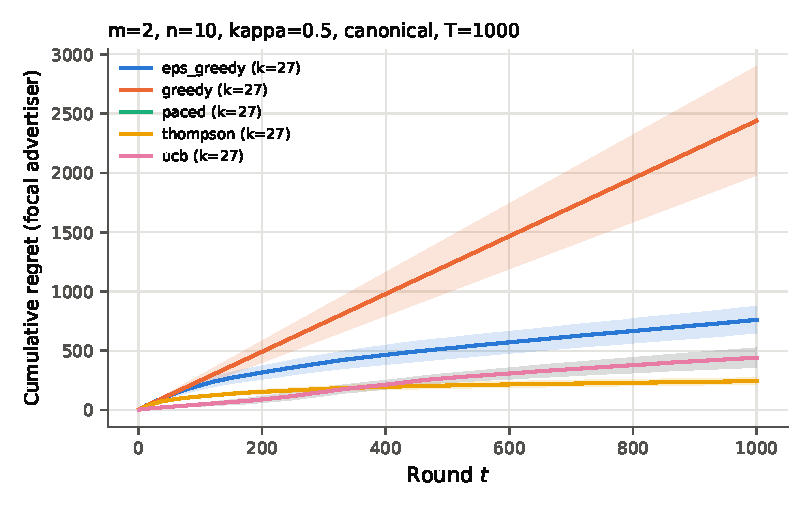
\includegraphics[width=\linewidth]{figures/tier2_curves_cum_regret.pdf}\\[-0.2em]
  {\small (a) $T=10^3$}
\end{minipage}\hfill
\begin{minipage}[t]{0.495\linewidth}\centering
  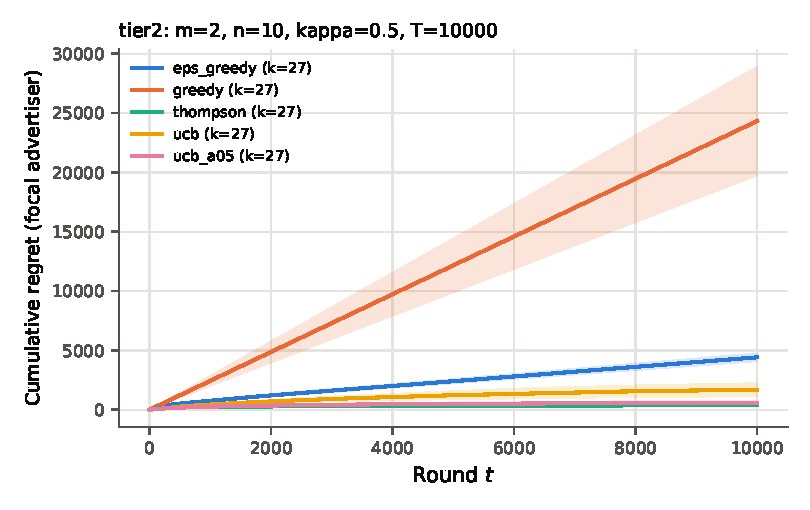
\includegraphics[width=\linewidth]{figures/tier2_long_cum_regret_m2_n10.pdf}\\[-0.2em]
  {\small (b) $T=10^4$}
\end{minipage}
\caption{Tier 2: cumulative regret of the learning advertiser for $m=2$, $n=10$, $\kappa=0.5$; mean and
$95\%$ band over the $27$ seeds with a pure equilibrium. Greedy grows linearly; TS flattens fastest. In (a)
the paced curve lies exactly under UCB.}
\label{fig:t2}
\end{figure}

\paragraph{H3: budgets do not slow learning.} Table~\ref{tab:kappa} breaks results down by budget level.
TS's regret per round is flat in $\kappa$ ($0.45$--$0.53$), and UCB's is largest at $\kappa=1$ ($1.17$, $0.81$, $1.64$, $3.38$
for $\kappa=0.1,0.25,0.5,1$), plausibly because a larger budget lets an optimistic learner buy more
exploratory impressions each round. The efficiency loss at small $\kappa$ is already present in $b^\ast$
(Table~\ref{tab:t1}), and in Tier~3 TS tracks the Tier-1 efficiency within $0.01$--$0.04$ at every $\kappa$.
\textbf{H3 is not supported as stated}: scarce budgets lower efficiency through the equilibrium, not
through slower learning.

\begin{table}[t]
\caption{Effect of the budget level, canonical budgets, $T=10^3$. Top: Tier-2 regret per round. Bottom:
Tier-3 final efficiency compared with the Tier-1 reference.}
\label{tab:kappa}
\centering\small
\begin{tabular}{@{}llcccc@{}}
\toprule
 & Nominal $\kappa$ & $0.1$ & $0.25$ & $0.5$ & $1.0$\\
\midrule
Tier 2 regret / round & Thompson sampling & $0.48$ & $0.45$ & $0.53$ & $0.50$\\
 & UCB, $\alpha=0.5$ & $0.55$ & $0.47$ & $0.86$ & $1.02$\\
 & UCB, $\alpha=2$ & $1.17$ & $0.81$ & $1.64$ & $3.38$\\
 & $\epsilon$-greedy & $0.71$ & $1.05$ & $1.47$ & $1.64$\\
 & Greedy & $1.11$ & $2.94$ & $3.86$ & $3.91$\\
\midrule
Efficiency & Tier-1 reference $b^\ast$ & $0.32$ & $0.52$ & $0.73$ & $0.73$\\
 & Tier 3, known-$f$ control & $0.30$ & $0.49$ & $0.68$ & $0.66$\\
 & Tier 3, Thompson sampling & $0.31$ & $0.51$ & $0.69$ & $0.72$\\
 & Tier 3, UCB, $\alpha=2$ & $0.19$ & $0.31$ & $0.42$ & $0.48$\\
\bottomrule
\end{tabular}
\end{table}

\subsection{Tier 3 (H2): concurrent learning keeps the market away from $b^\ast$}
Table~\ref{tab:t3} and Figure~\ref{fig:t3} report what happens when every advertiser learns. The final
equilibrium gap grows with $m$ for every learner except greedy, which is stuck far from equilibrium at
every $m$, as H2 predicts. The control row shows how much of this is due to learning. Even with known $f$,
simultaneous best response does not settle on $b^\ast$. Each advertiser reacts to bids that the others are
changing in the same round, so play cycles (the control's gap in Figure~\ref{fig:t3}(a) alternates between
high and low values from round to round); its final gap is $0.76/1.42/2.37$ for $m=2/3/5$. TS ends
slightly \emph{closer} to equilibrium for $m\le3$ ($0.67/1.25/2.48$), plausibly because random posterior
samples desynchronise the advertisers' reactions. UCB ($\alpha=2$) and $\epsilon$-greedy stay $2$--$5$ units
away, and greedy locks into a wrong profile with efficiency $0.29$. With TS the price of learning is small:
efficiency falls by $0.02$ and revenue by $2.6$ per round, while advertisers' total profit \emph{rises} by
$0.3$, because concurrent bidding pushes prices down (the control shows the same pattern). Over
$T=10^4$ the gap keeps shrinking for TS ($0.40\to0.29$ at $m=2$, $n=10$) and UCB ($1.64\to0.77$), but not for
greedy ($3.47\to3.47$) or $\epsilon$-greedy ($1.29\to1.30$), whose exploration never decays.
\textbf{H2 is supported}, with the qualification that concurrent adaptation alone already produces most of
the gap.

\begin{table}[t]
\caption{Tier 3 (all advertisers run the same learner), canonical budgets, $T=10^3$: final equilibrium gap
by $m$, final efficiency, and price of learning (Tier-1 value minus final value, positive is a loss)
averaged over the grid. The Tier-1 reference has efficiency $0.58$ and revenue $18.9$ per round.}
\label{tab:t3}
\centering\small
\begin{tabular}{@{}lccccccc@{}}
\toprule
 & \multicolumn{3}{c}{Final gap $\varepsilon$} & & \multicolumn{3}{c}{Price of learning}\\
\cmidrule{2-4}\cmidrule{6-8}
Learner & $m=2$ & $m=3$ & $m=5$ & $\Eff$ & Efficiency & Revenue & Total profit\\
\midrule
Known-$f$ best response (control) & $0.76$ & $1.42$ & $\mathbf{2.37}$ & $0.53$ & $0.04$ & $4.0$ & $-0.5$\\
Thompson sampling & $\mathbf{0.67}$ & $\mathbf{1.25}$ & $2.48$ & $\mathbf{0.56}$ & $\mathbf{0.02}$ & $\mathbf{2.6}$ & $-0.3$\\
UCB, $\alpha=0.5$ & $1.21$ & $2.38$ & $4.04$ & $0.43$ & $0.14$ & $3.0$ & $3.9$\\
UCB, $\alpha=2$ & $2.32$ & $3.67$ & $4.93$ & $0.35$ & $0.23$ & $2.8$ & $7.7$\\
$\epsilon$-greedy & $2.17$ & $3.36$ & $4.82$ & $0.46$ & $0.12$ & $3.3$ & $3.2$\\
Greedy & $4.79$ & $4.82$ & $4.42$ & $0.29$ & $0.29$ & $9.9$ & $4.5$\\
\bottomrule
\end{tabular}
\end{table}

\begin{figure}[t]
\centering
\begin{minipage}[t]{0.495\linewidth}\centering
  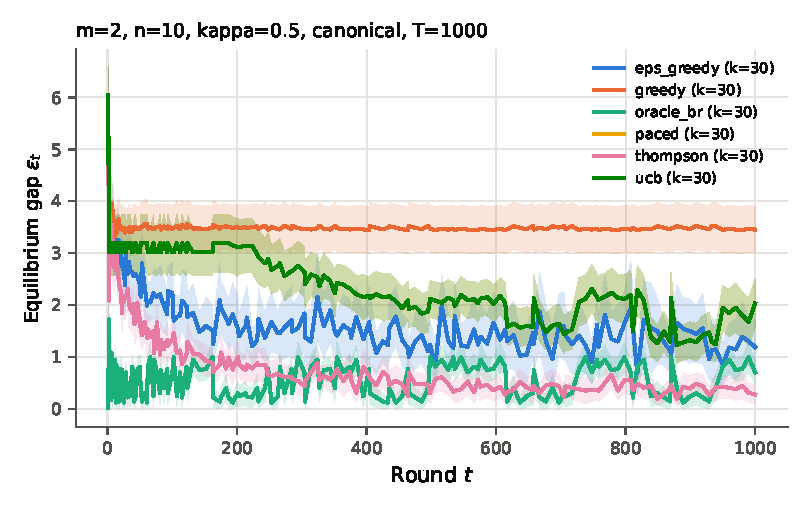
\includegraphics[width=\linewidth]{figures/tier3_curves_eq_gap.pdf}\\[-0.2em]
  {\small (a) Equilibrium gap $\varepsilon_t$}
\end{minipage}\hfill
\begin{minipage}[t]{0.495\linewidth}\centering
  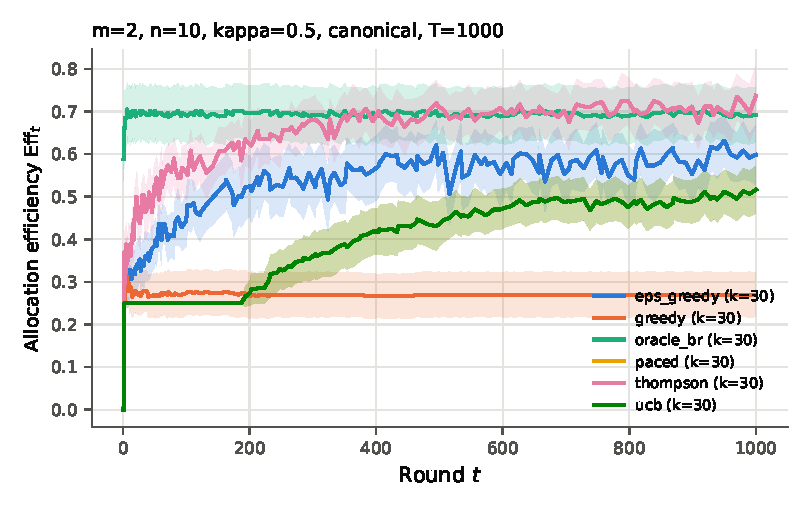
\includegraphics[width=\linewidth]{figures/tier3_curves_efficiency.pdf}\\[-0.2em]
  {\small (b) Allocation efficiency $\Eff_t$}
\end{minipage}
\caption{Tier 3 learning curves for $m=2$, $n=10$, $\kappa=0.5$, canonical budgets; mean and $95\%$ band over
$30$ seeds. \texttt{oracle\_br} is the known-$f$ control. TS reaches the control's efficiency after about
$400$ rounds, and its gap then stays mostly below the control's oscillating gap; greedy freezes after a few rounds.}
\label{fig:t3}
\end{figure}

\subsection{Robustness to the budget structure}
Table~\ref{tab:robust} repeats the comparison under the two other budget structures. The discounted variant
($\gamma=0.999$) puts more weight on early rounds but changes no conclusion: TS again has the lowest regret in
all $47$ Tier-2 cells and the smallest exponent. Under a \emph{cumulative} campaign budget the picture changes.
Myopic learners spend as if the budget reset every round. Against the fluid benchmark TS still has the
lowest mean final regret ($1180$) and wins $26$ of $47$ cells. The paced learner wins $13$ cells and is the
only one still earning substantially at the end of the campaign: $3.42$ per round over the last $10\%$ of
rounds, against at most $1.91$ for the myopic learners and $0$ for UCB, which spends its budget too early. In Tier~3 the paced agent has the smallest final gap
($2.52/3.21/3.89$ for $m=2/3/5$, against $4.1$--$5.0$ for TS) and the smallest revenue loss ($5.9$ against
$10.0$--$13.4$). With a single campaign budget, pacing matters more than the choice of bandit index. One
caveat: the fixed-$b^\ast$ opponents in Tier~2 do not pace either and can run out of budget mid-campaign, so
under this structure the learner's market is not stationary.

\begin{table}[t]
\caption{Other budget structures, $T=10^3$, grid means. Discounted: Tier-2 regret exponent. Cumulative
(campaign budget $0.5\,TB_i$): Tier-2 final regret against the fluid LP benchmark, learner profit per round
over the last $10\%$ of rounds, and cells won (lowest regret among all five learners); Tier-3 final gap for $m=2/3/5$ and revenue loss.}
\label{tab:robust}
\centering\small
\begin{tabular}{@{}lcccccc@{}}
\toprule
 & Discounted & \multicolumn{3}{c}{Cumulative, Tier 2} & \multicolumn{2}{c}{Cumulative, Tier 3}\\
\cmidrule(lr){2-2}\cmidrule(lr){3-5}\cmidrule(l){6-7}
Learner & Exponent & Regret & Profit / round & Wins & Gap $m=2/3/5$ & Revenue loss\\
\midrule
Thompson sampling & $\mathbf{0.25}$ & $\mathbf{1180}$ & $1.49$ & $\mathbf{26}$ & $4.98/4.76/4.09$ & $11.9$\\
UCB, $\alpha=2$ & $0.59$ & $2912$ & $0.00$ & $1$ & $7.17/4.83/3.98$ & $10.0$\\
$\epsilon$-greedy & $0.51$ & $1402$ & $1.76$ & $6$ & $5.12/5.35/5.34$ & $11.5$\\
Greedy & $0.63$ & $2295$ & $1.91$ & $1$ & $4.68/4.67/4.59$ & $13.4$\\
Budget-paced & $0.59$ & $1378$ & $\mathbf{3.42}$ & $13$ & $\mathbf{2.52/3.21/3.89}$ & $\mathbf{5.9}$\\
\bottomrule
\end{tabular}
\end{table}

% =====================================================================
\section{Discussion, limitations and future work}\label{sec:discussion}
Three findings stand out. \emph{Learning against a fixed market is cheap}: the knapsack oracle does the
combinatorial work and the bandit index only ranks users. \emph{Concurrent adaptation, not learning, is the main
obstacle to equilibrium}: known-$f$ best response already cycles. \emph{Budget scarcity acts through the
equilibrium}, not through slower learning.

\paragraph{Deviations from the proposal.} (i)~We use $v=5$ instead of $v=1$ (Section~\ref{sec:model}).
(ii)~For small games we search all pure profiles exhaustively rather than running Lemke--Howson on mixed
strategies, since Tiers~2 and~3 need a pure reference profile; instances without one are reported and
excluded from Tier~2. (iii)~The cumulative budget is $0.5\,TB_i$ with a per-round cap of $B_i$, so pacing is
necessary but the per-round knapsack is unchanged.

\paragraph{Limitations.} Integer bids force $v=5$, and a finer bid grid could change the equilibria. Tier~2
keeps only seeds with a pure $b^\ast$; half of the $292$ it drops come from $m=5$, $n\ge20$. Rerunning it on
all $1440$ seeds, with opponents fixed at the last BRD profile where no pure equilibrium exists, leaves the
ranking unchanged: TS has the lowest regret in all $48$ cells, and on the dropped seeds alone in $21$ of
$22$ cells ($0.88$ regret per round against $3.31$ for UCB). The regret exponent is a mean of
per-seed slopes and is unstable when $\Reg_{T/10}\approx0$: for UCB ($\alpha=2$) it exceeds $1$ in two cells
($1.24$ at $m=2$, $n=10$, $\kappa=0.5$; median $1.03$) because some seeds pay almost no regret before
$t=100$, although mean regret per round falls from a peak of $0.63$ to $0.30$. The learner sees the highest competing bid
(Assumption~2); with win/loss feedback only it would also have to learn prices. Click rates are synthetic and
independent across users and advertisers.

\paragraph{Future work.} The two most direct extensions from the proposal are contextual click models that
share information across similar users (a LinUCB-style index~\citep{li2010contextual}) and learning the
winning-price distribution from win/loss outcomes alone, which turns the per-round problem into a
multiple-choice knapsack.

\paragraph{Code, reproducibility and demo.} Repository:
\url{https://github.com/VivekRaj2708/FAI-Group22}. \texttt{python run\_tests.py} runs the $54$ tests;
\texttt{python run\_evaluation.py sweep \dots} then \texttt{report} regenerates every figure and per-cell table
(commands in the README); \texttt{python report\_numbers.py} recomputes every number in this report; and
\texttt{python run\_demo.py} (or \texttt{demo/index.html}) animates a market with the project's own agents.

% =====================================================================
\section{Contribution}\label{sec:contrib}
Table~\ref{tab:contrib} lists each member's assigned task (from the proposal), what they committed (from the Git
history) and whether the task was fulfilled. The proposal was written jointly; all work was merged through pull requests \#1--\#5.

\begin{table}[h]
\caption{Assigned tasks (from the proposal), delivered code (from the commit history) and status.}\label{tab:contrib}
\centering\footnotesize
\begin{tabularx}{\linewidth}{@{}>{\raggedright\arraybackslash}p{2.1cm}>{\raggedright\arraybackslash}X>{\raggedright\arraybackslash}X>{\raggedright\arraybackslash}p{1.45cm}@{}}
\toprule
Member & Assigned task & Delivered (commits) & Status\\
\midrule
Vivek Raj & Tier-1 known-$f$ baseline: knapsack DP best response, equilibrium computation, reference
$b^\ast$ and $p^\ast$ &
Auction engine and instance generator (\texttt{src/env/}); knapsack DP, best-response dynamics, fictitious
play, exhaustive pure-profile search and social planner (\texttt{src/tier1/}); \texttt{run\_tier1.py}; Tier-1
tests; proposal source and project setup & Fulfilled\\
Anvit Aggarwal & Tier-2 learners (UCB, TS, greedy baselines) with regret evaluation, and the budget-paced
variant for cumulative budgets & Shared agent interface (\texttt{src/agents/base.py}); UCB, TS, greedy,
$\epsilon$-greedy and dual-paced learners and the single-learner simulation (\texttt{src/tier2/});
\texttt{run\_tier2.py}; Tier-2 tests & Fulfilled\\
Eshaan Ashish Jaiswal & Tier-3 simulator with all advertisers learning; convergence data as $m$ and $n$ vary &
Multi-agent simulator, convergence-rate and cycling analysis, price of learning (\texttt{src/tier3/});
Tier-1 knapsack and equilibrium agents; \texttt{run\_tier3.py}, \texttt{collect\_convergence\_logs.py},
test runner \texttt{run\_tests.py}; Tier-3 tests & Fulfilled\\
Gella Naga Sai Krishna & Shared evaluation harness (metrics, plots); sensitivity study over round structures
and budget levels; final report & Evaluation harness (\texttt{src/eval/},
\texttt{run\_evaluation.py}), agent registry; all sweeps in \texttt{results/}; \texttt{report\_numbers.py};
live demo; this report and README & Fulfilled\\
\bottomrule
\end{tabularx}
\end{table}

% =====================================================================
\footnotesize
\begin{thebibliography}{99}
\setlength{\itemsep}{0pt}
\bibitem{kellerer2004knapsack} H.~Kellerer, U.~Pferschy, and D.~Pisinger. \emph{Knapsack Problems}. Springer, 2004.
\bibitem{auer2002finite} P.~Auer, N.~Cesa-Bianchi, and P.~Fischer. Finite-time analysis of the multiarmed bandit problem. \emph{Machine Learning}, 47(2--3):235--256, 2002.
\bibitem{lattimore2020bandit} T.~Lattimore and C.~Szepesv{\'a}ri. \emph{Bandit Algorithms}. Cambridge University Press, 2020.
\bibitem{krishna2009auction} V.~Krishna. \emph{Auction Theory}. Academic Press, 2nd edition, 2009.
\bibitem{balseiro2019learning} S.~R.~Balseiro and Y.~Gur. Learning in repeated auctions with budgets: Regret minimization and equilibrium. \emph{Management Science}, 65(9):3952--3968, 2019.
\bibitem{han2020optimal} Y.~Han, Z.~Zhou, and T.~Weissman. Optimal no-regret learning in repeated first-price auctions. arXiv:2003.09795, 2020.
\bibitem{badanidiyuru2013bandits} A.~Badanidiyuru, R.~Kleinberg, and A.~Slivkins. Bandits with knapsacks. In \emph{Proc.\ IEEE FOCS}, pages 207--216, 2013.
\bibitem{chen2013combinatorial} W.~Chen, Y.~Wang, and Y.~Yuan. Combinatorial multi-armed bandit: General framework and applications. In \emph{Proc.\ ICML}, pages 151--159, 2013.
\bibitem{nash1951noncooperative} J.~Nash. Non-cooperative games. \emph{Annals of Mathematics}, 54(2):286--295, 1951.
\bibitem{thompson1933likelihood} W.~R.~Thompson. On the likelihood that one unknown probability exceeds another in view of the evidence of two samples. \emph{Biometrika}, 25(3--4):285--294, 1933.
\bibitem{agrawal2012analysis} S.~Agrawal and N.~Goyal. Analysis of {T}hompson sampling for the multi-armed bandit problem. In \emph{Proc.\ COLT}, 2012.
\bibitem{agrawal2014bandits} S.~Agrawal and N.~R.~Devanur. Bandits with concave rewards and convex knapsacks. In \emph{Proc.\ ACM EC}, 2014.
\bibitem{li2010contextual} L.~Li, W.~Chu, J.~Langford, and R.~E.~Schapire. A contextual-bandit approach to personalized news article recommendation. In \emph{Proc.\ WWW}, pages 661--670, 2010.
\end{thebibliography}

\end{document}
